%----------------------------------------------------------------------------------------
% DOCUMENT CONFIGURATIONS
%----------------------------------------------------------------------------------------

\documentclass[
11pt, % The default document font size, options: 10pt, 11pt, 12pt
oneside, % Two side (alternating margins) for binding by default, uncomment to switch to one side
english, % other languages available
singlespacing, % Single line spacing, alternatives: onehalfspacing or doublespacing
%draft, % Uncomment to enable draft mode (no pictures, no links, overfull hboxes indicated)
%nolistspacing, % If the document is onehalfspacing or doublespacing, uncomment this to set spacing in lists to single
%liststotoc, % Uncomment to add the list of figures/tables/etc to the table of contents
%toctotoc, % Uncomment to add the main table of contents to the table of contents
]{McMasterThesis} % The class file specifying the document structure


%----------------------------------------------------------------------------------------
% Import packages here
%----------------------------------------------------------------------------------------
\usepackage[utf8]{inputenc} % Required for inputting international characters
\usepackage[T1]{fontenc} % Output font encoding for international characters

\usepackage{lmodern} % could change font type by calling a different package
\usepackage{lastpage} % count pages
\usepackage{siunitx} % for scientific units (micro-liter, etc)
\setcounter{tocdepth}{2} % so that only section and sub sections appear in Table of Contents. Remove or set depth to 3 to include sub-sub-sections

\usepackage{rotating} % rotating table and figure
\usepackage[T1]{fontenc}
\usepackage[utf8]{inputenc}

 
%% Text box -----------------------
\usepackage{mdframed} % text box
% all 4 borders
\newmdenv{allfour}

% just top and bottom
\newmdenv[leftline=false,rightline=false]{topbot}

% just left and bottom
\newmdenv[topline=false,rightline=false]{leftbot}

\usepackage{blindtext}

%----------------------------------------------------------------------------------------
% Chapter wise Citations
%----------------------------------------------------------------------------------------
\usepackage[sectionbib]{natbib}
\usepackage{chapterbib}
%%% Uncomment if you change the bibliography heading/title
\renewcommand{\bibname}{References}

%%% Uncomment if you want to include the bibliographies at the end of each chapter in the table of contents.  
\usepackage[nottoc]{tocbibind}


%----------------------------------------------------------------------------------------
% Collect all your header information from the chapters here, things like acronyms, custom commands, necessary packages, etc. 
%----------------------------------------------------------------------------------------
\usepackage{parskip} %this will put spaces between paragraphs
\setlength{\parindent}{15pt} % this will create and indent on all but the first paragraph of each section. 
% should maybe change to glossaries package
\usepackage{acro}
\DeclareAcronym{est}{
	short = EST,
	long  = expressed sequence tags
}

\DeclareAcronym{Xl}{
	short = \textit{X.~laevis},
	long  = \textit{Xenopus~laevis}
}
\DeclareAcronym{Xg}{
	short = \textit{X.~gilli},
	long  = \textit{Xenopus~gilli}
}

\usepackage{etoolbox}
\preto\chapter{\acresetall} % resets acronyms for each chapter

\usepackage{xspace} %helps spacing with custom commands. 
\newcommand{\oddname}{{\sc SoME goOfY LonG ThiNg With an AwkWarD NAme}\xspace}


\usepackage{pgfplotstable} % a much better way to handle tables
\pgfplotsset{compat=1.12}


%----------------------------------------------------------------------------------------
%	THESIS INFORMATION
%----------------------------------------------------------------------------------------

% Big Data Clustering Models and Applications in Research and Subscription-based Platforms

\thesistitle{Your Thesis Title} % Your thesis title, print it elsewhere with \ttitle


\supervisor{xxxx xxxx} % Your supervisor's name, print it elsewhere with \supname
\examiner{} % Your examiner's name, print it elsewhere with \examname
\degree {Ph.D.} % Your degree name, print it elsewhere with \degreename
\subjectarea{Computational Science and Engineering} % Your degree area name, print it elsewhere with \area
\author{xxxxxx xxxxx} % Your name, print it elsewhere with \authorname
\addresses{} % Your address, print it elsewhere with \addressname

\subject{Computational Science \& Engineering} % Your subject area, print it elsewhere with \subjectname
\keywords{} % Keywords for your thesis, print it elsewhere with \keywordnames
\university{\href{http://www.mcmaster.ca/}{McMaster University}} % Your university's name and URL, print it elsewhere with \univname
\department{\href{https://computational.mcmaster.ca/}{Computational Science \& Engineering}} % Your department's name and URL, print it elsewhere with \deptname
\group{\href{http://www.science.mcmaster.ca/}{Research Group Name}} % Your research group's name and URL, print it elsewhere with \groupname
\faculty{\href{http://www.science.mcmaster.ca/}{Faculty of Science}} % Your faculty's name and URL, print it elsewhere with \facname

% this sets up hyperlinks
\hypersetup{pdftitle=\ttitle} % Set the PDF's title to your title
\hypersetup{pdfauthor=\authorname} % Set the PDF's author to your name
\hypersetup{pdfkeywords=\keywordnames} % Set the PDF's keywords to your keywords



%----------------------------------------------------------------------------------------
% Begin document
%----------------------------------------------------------------------------------------
\begin{document}
\frontmatter

\frontmatter % Use roman page numbering style (i, ii, iii, iv...) for the pre-content pages

\pagestyle{plain} % Default to the plain heading style until the thesis style is called for the body content

%----------------------------------------------------------------------------------------
%	Half Title (lay title)
%----------------------------------------------------------------------------------------
%\begin{halftitle} % could not get this environment working
%\vspace*{\fill}
\vspace{6cm}
\begin{center}
A short 60 character title % ideally, but it doesn't seem to matter
\end{center}
%\vspace*{\fill}
\pagenumbering{gobble} % leave this here, McMaster doesn't want this page numbered
%\end{halftitle}
\clearpage

%----------------------------------------------------------------------------------------
%	TITLE PAGE
%----------------------------------------------------------------------------------------
\pagenumbering{gobble}
\begin{center}

\vfill
\textsc{\Large \ttitle} \\

\vfill
By \authorname, \\%% -----> List prior degrees after comma  <----

 \vfill
{\large \textit{A Thesis Submitted to the School of Graduate Studies in the Partial Fulfillment of the Requirements for the Degree of}}\\

\vfill
{\large  \degreename}\\ \vspace{15pt}
{\large  in}\\ \vspace{15pt}
{\large  \subjectareaname}\\
\vfill
\vfill
{\large \univname\, \\ Hamilton, Ontario}\\[4cm] % replace \today with the submission date


{\copyright\, Copyright by \authorname\, \today}\\[4cm] % replace \today with the submission date

\end{center}

%----------------------------------------------------------------------------------------
%	Descriptive note numbered ii
%----------------------------------------------------------------------------------------
% Need to add below info
\newpage
\pagenumbering{roman} % leave to turn numbering back on
\setcounter{page}{2} % leave here to make this page numbered ii, a Grad School requirement

\noindent % stops indent on next line
\univname \\ 
\degreename\, (\the\year) \\
Hamilton, Ontario (\deptname) \\[1.5cm]
TITLE: \ttitle 
\\ \\
AUTHOR:\\ \authorname\,\\ 
School of Computational Science and Engineering, McMaster University %list previous degrees  
\\ \\
SUPERVISOR:\\ \supname\,\\
Title and Department, , \\
McMaster University
\\ 
\\
SUPERVISORY COMMITTEE CHAIR: \\ xxx xxxx,\\
Title and Department, , \\
McMaster University 
\\
\\
SUPERVISORY COMMITTEE MEMBERS: \\xxxx xxxxx\\ 
Title and Department, \\
McMaster University
\\
\\
xxx xxxxx\\ 
Title and Department, , \\
McMaster University  
\\
\\
NUMBER OF PAGES: \pageref{lastoffront}, \pageref{LastPage}  % put in iv and number

\clearpage



%----------------------------------------------------------------------------------------
%	ABSTRACT PAGE
%----------------------------------------------------------------------------------------

\section*{\Huge Abstract} 
\addchaptertocentry{Abstract}
% Type your abstract here. 
An abstract! 
\clearpage
%----------------------------------------------------------------------------------------
%	ACKNOWLEDGEMENTS
%----------------------------------------------------------------------------------------

\begin{acknowledgements}
\addchaptertocentry{\acknowledgementname} % Add the acknowledgements to the table of contents

The acknowledgements and the people to thank go here, don't forget to include your project adviser\ldots

\end{acknowledgements}

%----------------------------------------------------------------------------------------
%	LIST OF CONTENTS/FIGURES/TABLES PAGES
%----------------------------------------------------------------------------------------

\tableofcontents % Prints the main table of contents

\listoffigures % Prints the list of figures

\listoftables % Prints the list of tables


%----------------------------------------------------------------------------------------
%	DECLARATION PAGE
%----------------------------------------------------------------------------------------

\begin{declaration}
\addchaptertocentry{\authorshipname}

\noindent I, Dewan F. Wahid, declare that this thesis titled, Big Data Clustering Models and Applications in Research and Subscription-based Platforms and the work presented in it are my own. I confirm that

\begin{itemize} 
\item List each chapter
\item and what you have done for it
\end{itemize}
 
\end{declaration}

%----------------------------------------------------------------------------------------
% The following bit is just here to make sure we end up on a new page and get the total number of roman numeral
\label{lastoffront}
\clearpage
% make sure this command is on the last of your frontmatter pages, i.e. only this command, a \clearpage then \mainmatter
% should be fine without modification
%----------------------------------------------------------------------------------------

%----------------------------------------------------------------------------------------
%	THESIS CONTENT - CHAPTERS
%----------------------------------------------------------------------------------------

\mainmatter
\chapter{Introduction}

\section{Section Heading}
Here's a citation! \citep{bansal2004correlation}

%\bibliographystyle{unsrtnat}  %% For numerical citations remember to pass "numbers" option to natbib
\bibliographystyle{dcu}
\bibliography{Bibliography}
% remember to set these at the start of each chapter
\chapter{Title of Chapter 2}
\label{chapt2} 

%%%%%%%%%%%%%%%%%%
\vspace{60pt}


%%% ---------------------
%%% Publication citation 
%%% ---------------------
The content of this chapter is a second revision of the manuscript text for publication under the following citation:\\
% \vspace{20pt}

\begin{topbot}
Heider, F. (1946). Attitudes and cognitive organization. The Journal of psychology, 21(1), 107-112.
\end{topbot}

\newpage


%%% ---------------------
%%% Paper title
%%% ---------------------
\begin{center}
    \Large \textbf{Your first paper tile}
\end{center}

\vspace{40pt}

%%% ---------------------
%%% Authors
%%% ---------------------
\begin{center}
First Author\\
\textit{School of Computational Science and Engineering}\\
\textit{McMaster University, Hamilton, ON, Canada}\\
\textit{Email: \href{mailto:xxxxx@mcmaste.ca}{xxxx@mcmaste.ca}}

\vspace{10pt}

Second Author\\
\textit{DeGroote School of Business}\\
\textit{McMaster University}\\
\textit{Email: \href{mailto:xxxx@mcmaster.ca}{xxxx@mcmaster.ca}}

\end{center}


\vspace{30pt}

\begin{onehalfspacing}
%%-----------------------

\section*{\centering Abstract}
First paper abastract.


\paragraph{\textit{\textbf{Keywords:}}} \textit{keyword, keyword2} 
 


\vspace{20pt} 

\section{Section Title 2}
\label{s-1-cc}
Introduction  \citet{heider1946attitudes} 
\citep{doreian1996partitioning}

\subsection{Section Title 2}

\blindtext

\subsubsection{Section Title 3}
\blindtext 

%% FIGURE 01 -------
\begin{figure}[h]
    \centering
    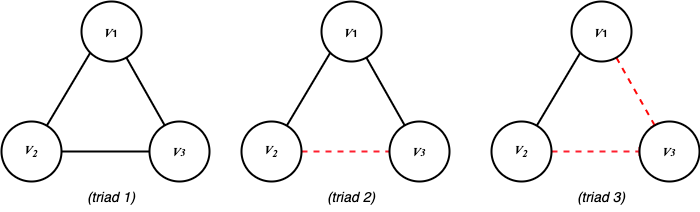
\includegraphics[width=0.75\textwidth]{Figs/Chapter2/fig_exmp.png}
    \caption{Caption.}
\label{fig:1-cc}  
\end{figure}



\end{onehalfspacing}



\bibliographystyle{dcu}
\bibliography{Bibliography}


\include{chap3}
\include{chap4}
\include{chap5}
\include{chap6}

%----------------------------------------------------------------------------------------
%	THESIS CONTENT - APPENDICES
%----------------------------------------------------------------------------------------

\appendix % Cue to tell LaTeX that the following "chapters" are Appendices
\renewcommand{\thetable}{A\arabic{chapter}.\arabic{table}} % adds an A to table names in appendix (Table A1.1, A1.2...)
\renewcommand{\thefigure}{A\arabic{chapter}.\arabic{figure}} % same for figures
\renewcommand{\thesection}{A\arabic{section}}

% Include the appendices of the thesis as separate files from the Appendices folder
% \input{Appendix/Supp_Chap3.tex}


% \backmatter
% %% A list of publications can be created using this approach
% \include{ownpubs}

\end{document}
